%%%%%%%%%%%%%%%%%%%%%%%%%%%%%%%%%%%%%%%%%
% fphw Assignment
% LaTeX Template
% Version 1.0 (27/04/2019)
%
% This template originates from:
% https://www.LaTeXTemplates.com
%
% Authors:
% Class by Felipe Portales-Oliva (f.portales.oliva@gmail.com) with template 
% content and modifications by Vel (vel@LaTeXTemplates.com)
%
% Template (this file) License:
% CC BY-NC-SA 3.0 (http://creativecommons.org/licenses/by-nc-sa/3.0/)
%
%%%%%%%%%%%%%%%%%%%%%%%%%%%%%%%%%%%%%%%%%

%----------------------------------------------------------------------------------------
%	PACKAGES AND OTHER DOCUMENT CONFIGURATIONS
%----------------------------------------------------------------------------------------

\documentclass[
	12pt, % Default font size, values between 10pt-12pt are allowed
	%letterpaper, % Uncomment for US letter paper size
	%spanish, % Uncomment for Spanish
]{fphw}

% Template-specific packages
\usepackage[utf8]{inputenc} % Required for inputting international characters
\usepackage[T1]{fontenc} % Output font encoding for international characters
\usepackage{mathpazo} % Use the Palatino font

\usepackage{graphicx} % Required for including images

\usepackage{booktabs} % Required for better horizontal rules in tables

\usepackage{listings} % Required for insertion of code

\usepackage{enumerate} % To modify the enumerate environment

%----------------------------------------------------------------------------------------
%	ASSIGNMENT INFORMATION
%----------------------------------------------------------------------------------------

\title{Assignment \#1} % Assignment title

\author{Kunal Sunil Kasodekar} % Student name

\date{September 26th, 2022} % Due date

\institute{Arizona State University} % Institute or school name

\class{CSE 598 Advanced topics in machine learning security, privacy and fairness} % Course or class name

\professor{Chaowei Xiao} % Professor or teacher in charge of the assignment

%----------------------------------------------------------------------------------------

\begin{document}

\maketitle % Output the assignment title, created automatically using the information in the custom commands above

%----------------------------------------------------------------------------------------
%	ASSIGNMENT CONTENT
%----------------------------------------------------------------------------------------
\section*{Environment/Setup:}

WSL with Ubuntu 18.04 and Python 3.7 with the latest stable version of Pytorch is set up in a Conda virtual environment. The system has no GPU and makes use of an i5vPro 10 Gen CPU for training.
However, for faster iterations in training and attacking the model, resolving some bugs and prototyping I shifted to Colab for GPU Access. 
\newline
\underline{The Colab notebook link is}:
https://colab.research.google.com/drive/14HIPB1Ehj2qafuD28-L1m3Y58fdIpXKU?usp=sharing.
\textit{Errors were resolved using Colab and the bugs were fixed in the local codebase.}
The codebase is maintained using Git.

\section*{Submission Files/Format:}
The output file contains the codebase for the whole assignment including the ipynb notebook (\JupyterNotebookfroAssignment), py file, latex files used for submission and graphs.

\section*{Task 1: Train a Fashion-MNIST Classification}

Task 1 was to train the Fashion-MNIST Dataset with the following properties: 10 Classes, 50,000 training images, 10,000 validation images and 10,000 test images. Lenet-5 with the architecture given below is used to train the dataset. The Architecture was obtained from the class slides, 5th presentation, page 45. The questions and answer w.r.t to the task are given below:

\begin{problem}
	Architecture of the network:
\end{problem}
\begin{center}
	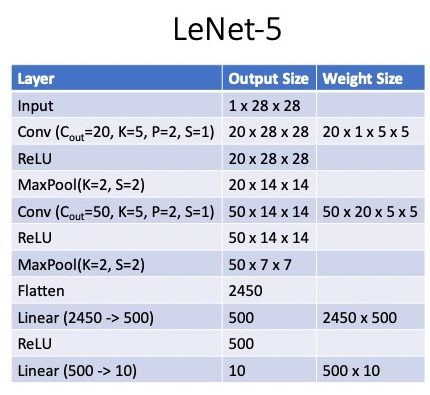
\includegraphics[width=0.45\columnwidth]{lenet5arch.png} 
\end{center}

\subsection*{Answer}

We make use of two 2D convolution layers, with:
\begin{itemize}
	\item Kernel Size = 5x5
	\item Stride = 1
	\item Padding = 2
	\item Activation Function: Relu
\end{itemize}

\noindent A max-pooling layer of size 2 and stride 2 is applied after the convolutions. After the convolutions and pooling the tensor is flattened and passed onto fully connected linear layers with Layer1 output=500 and layer2 output=10 (The number of classes to detect)
Relu is used as an Activation for all the trainable layers. 
Reference image for the Architecture is given above.
\newline

\noindent\textbf{Receptive Field of the network:} 

\begin{itemize}
	\item Inputs Local Receptive Field - 1x1
	\item Convolution 1 - 5x5
	\item Max Pool 1 - 10x10
	\item Convolution 2 - 14x14
	\item Max Pool 2 - 28x28
\end{itemize}

Hence Global Receptive field before the final FCN Layers is 28x28 implying that all the input pixels have been seen by the network.

\begin{problem}
	Optimizer and parameters:
\end{problem}

\subsection*{Answer}

After trying out all optimizers like SGD, RMSProp and Adam it was found that Adam gave the lowest cross-entropy loss on validation and the best accuracy on the validation dataset.
Other Optimal Hyperparameters including training parameters for the model are:

\begin{itemize}
	\item Learning Rate =  3e-4  
	\item Weight Decay = 1e-4
	\item Number of Epochs = 25 
	\item Batch size = 64 
\end{itemize} 

\begin{problem}
	Training and Validation Plots:
\end{problem}

\subsection*{Answer}

\begin{center}
	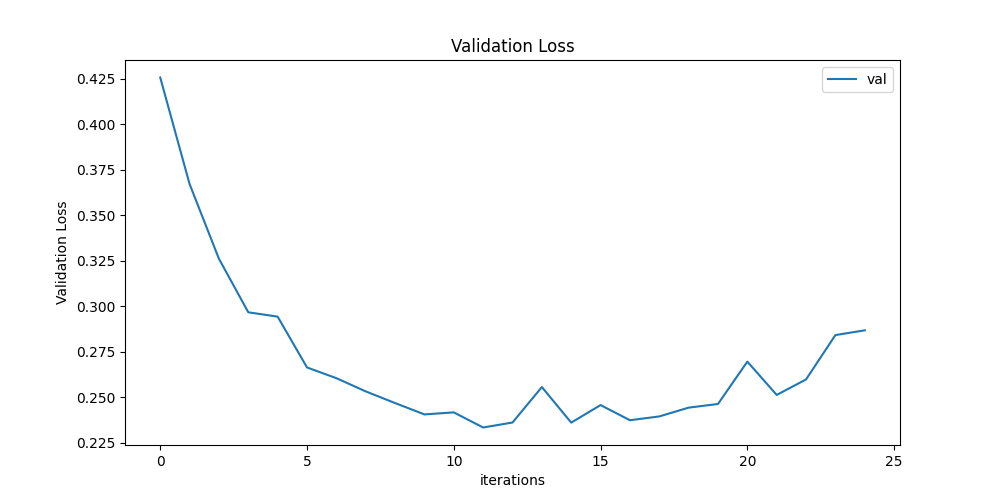
\includegraphics[width=0.85\columnwidth]{valloss.png} 
	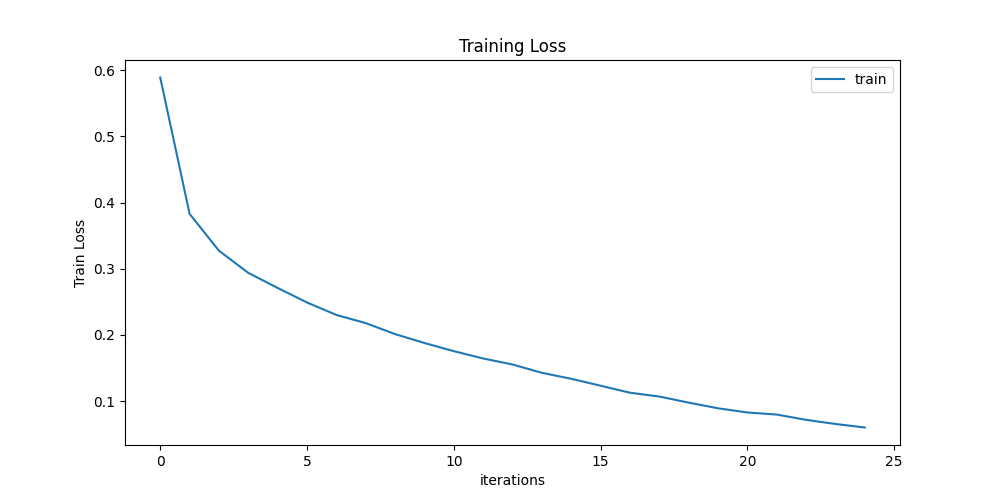
\includegraphics[width=0.85\columnwidth]{trainloss.png} 
\end{center}

\begin{problem}
	Best Model Accuracy:
\end{problem}

\subsection*{Answer}
After multiple experiments, the best accuracy on the Test Dataset is \textbf{91.83} Percent. The corresponding accuracy on the validation dataset is 92.25 Percent. The model is saved as Lenet5-FashionMNISTtrialv2.pt in the model folder using torch.save().

\section*{Task 2: Implement attacks for the Fashion-MNIST Classification}

\begin{problem}
	The Attack success rate of the FGSM attack (Epsilon = 25/255) on Test Dataset is:
\end{problem}

\subsection*{Answer}
The Attack success rate is: \textbf{86.36} Percent

\begin{problem}
	The Attack success rate of the PGD attack (Epsilon = 25/255) on different attack steps:
\end{problem}

\subsection*{Answer}
The Attack success rate for respective attack steps is:
\begin{itemize}
	\item 1: 20.19 Percent
	\item 2: 37.24 Percent
	\item 5: 75.05 Percent
	\item 10: \textbf{96.97} Percent
\end{itemize}


\begin{problem}
	Visualizing the 10-step PGD attack using 10 Adversarial Images (Test)
\end{problem}

\subsection*{Answer}

\begin{center}
	\caption{Random Images Predicted by LeNet}
	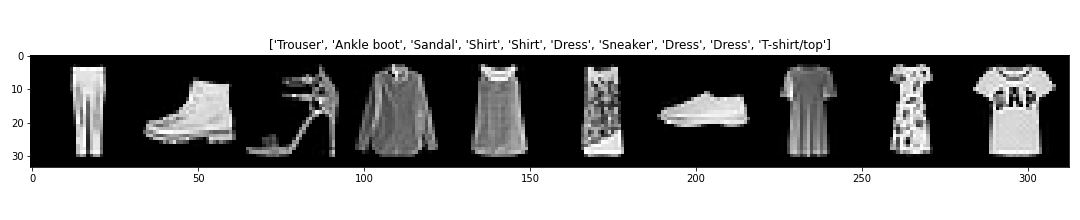
\includegraphics[width=0.95\columnwidth]{Plotclean_new.png} 
	\caption{PGD (n=10) Attacked Images with Predicted Labels}
	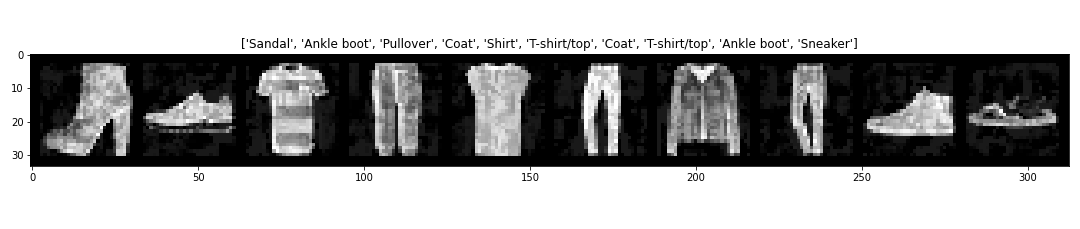
\includegraphics[width=0.95\columnwidth]{Plotadv_new_pred.png}
	\caption{PGD (n=10) Attacked Images with Actual Labels}
	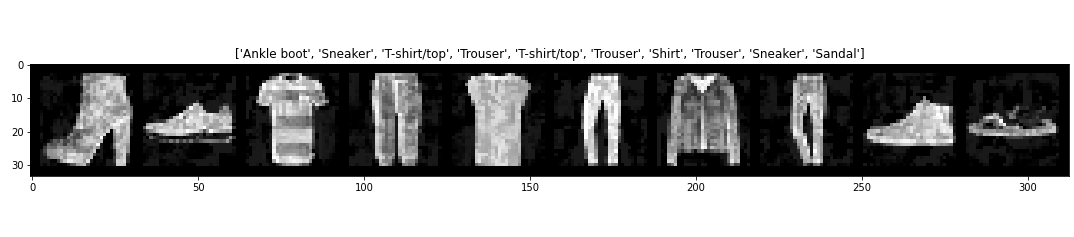
\includegraphics[width=0.95\columnwidth]{Plot_new_truelabel.png} 
\end{center}

\end{document}
